\documentclass[a4paper, 14pt]{extarticle}
\usepackage[utf8]{inputenc}
\usepackage[paper=a4paper, top=1cm, right=1cm, bottom=1.5cm, left=2cm]{geometry}
\usepackage{setspace}
\onehalfspacing

\usepackage{graphicx}
\graphicspath{{plots/}, {images/}}

\parindent=1.25cm

\usepackage{titlesec}

\titleformat{\section}
    {\normalsize\bfseries}
    {\thesection}
    {1em}{}

\titleformat{\subsection}
    {\normalsize\bfseries}
    {\thesubsection}
    {1em}{}

% Настройка вертикальных и горизонтальных отступов
\titlespacing*{\chapter}{0pt}{-30pt}{8pt}
\titlespacing*{\section}{\parindent}{*4}{*4}
\titlespacing*{\subsection}{\parindent}{*4}{*4}

\usepackage[square, numbers, sort&compress]{natbib}
\makeatletter
\bibliographystyle{unsrt}
\renewcommand{\@biblabel}[1]{#1.} 
\makeatother


\newcommand{\maketitlepage}[6]{
    \begin{titlepage}
        \singlespacing
        \newpage
        \begin{center}
            Министерство образования и науки Российской Федерации \\
            Федеральное государственное бюджетное образовательное \\
            учреждение высшего профессионального образования \\
            <<Волгоградский государственный технический университет>> \\
            #1 \\
            Кафедра #2
        \end{center}


        \vspace{14em}

        \begin{center}
            \large Семестровая работа #6 по дисциплине
            \\ <<#3>>
        \end{center}

        \vspace{5em}

        \begin{flushright}
            \begin{minipage}{.35\textwidth}
                Выполнила:\\#4
                \vspace{1em}\\
                Проверил:\\#5
                \\
                \\ Оценка \underline{\ \ \ \ \ \ \ \ \ \ \ \ \ \ \ \ }
            \end{minipage}
        \end{flushright}

        \vspace{\fill}

        \begin{center}
            Волгоград, \the\year
        \end{center}

    \end{titlepage}
    \setcounter{page}{2}
}

\newcommand{\maketitlepagewithvariant}[7]{
    \begin{titlepage}
        \singlespacing
        \newpage

        \begin{center}
            Министерство образования и науки Российской Федерации \\
            Федеральное государственное бюджетное образовательное \\
            учреждение высшего профессионального образования \\
            <<Волгоградский государственный технический университет>> \\
            #1 \\
            Кафедра #2
        \end{center}


        \vspace{8em}

        \begin{center}
            \large Семестровая работа #6 по дисциплине
            \\ <<#3>>
        \end{center}

        \vspace{1em}
        \begin{center}
            Вариант №#7
        \end{center}
        \vspace{4em}

        \begin{flushright}
            \begin{minipage}{.35\textwidth}
                Выполнила:\\#4
                \vspace{1em}\\
                Проверил:\\#5
                \\
                \\ Оценка \underline{\ \ \ \ \ \ \ \ \ \ \ \ \ \ \ \ }
            \end{minipage}
        \end{flushright}

        \vspace{\fill}

        \begin{center}
            Волгоград, \the\year
        \end{center}

    \end{titlepage}
    \setcounter{page}{2}
}

\input{../../../.preambles/10-russian}
\input{../../../.preambles/20-math}
\input{../../../.preambles/22-vectors}
\begin{document}
\maketitlepage{Факультет электроники и вычислительной техники}
{физики}{Электродинамика}{студентка группы Ф-369\\Слоква~В.~И.}
{доцент Грецов~М.~В.}{№1}

\renewcommand{\labelenumi}{\asbuk{enumi})}
\renewcommand{\v}{\mathrm{v}}

\newpage
%-------------------------------------------------------------------------------
\emph{79.} Пространство между двумя концентрическими сферами, радиусы которых
\( R_1 \) и \( R_2 \) (\( R_2 > R_1 \)), заряжено с объемной плотностью
\( \rho = \alpha/r^2 \). Найти полный заряд \( q \), потенциал \( \phi \) и
напряженность \( \vec{E} \) электрического поля. Рассмотреть предельный случай
\( R_2 \to R_1 \), считая при этом \( q = \mathrm{const} \).

\vspace*{2em}
\begin{figure}[h!]
    \center
    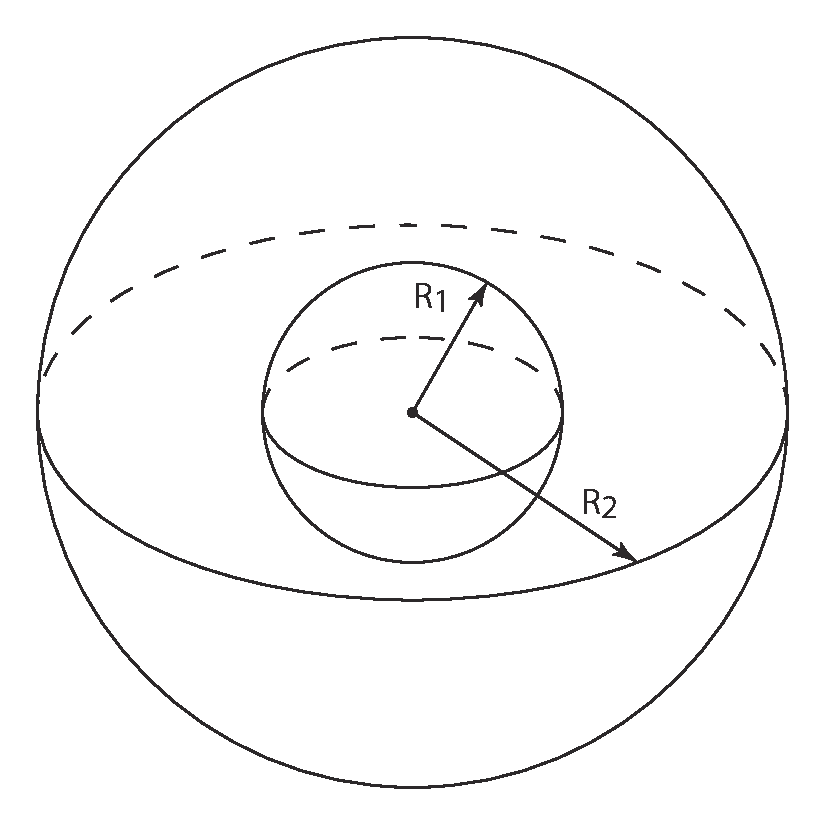
\includegraphics[width=.35\textwidth]{1-1}
\end{figure}
\emph{Решение:}

Найдем заряд \( q \):
\begin{align*}
    & V = \frac{4}{3}\pi r^3 \Rightarrow \d V = \frac{4}{3}\pi 3r^2\d r =
    4\pi r^2\d r; \\
    & q = \int\rho\d V = \int\limits_{R_1}^{R_2} 4\pi\rho r^2\d r = 4\pi \int
    \limits_{R_1}^{R_2} \frac{\alpha}{r^2} r^2\d r = 4\pi\alpha (R_2 - R_1).
\end{align*}

Если точка находится внутри сферы радиуса \( R_1 \), то есть \( r \le R_1 \), то
по теореме Гаусса: \( \oint \vec{E}\cdot\d\vec{S} = 4\pi q \), а так как
\( q = E(\vec{r})r^2 \), то \( \oint \vec{E}\cdot\d\vec{S} = 4\pi E r^2 \).

Но так как внутри сферы нет зарядов, то \( 4\pi E r^2 = 0 \), следовательно,
\( E = 0 \).

Из уравнения Пуассона \( \Delta\phi = -4\pi\rho \):
\begin{align*}
    & \frac{1}{r^2} \pder{}{r}\left(r^2\pder{\phi}{r}\right) =
    -4\pi\frac{\alpha}{r^2}; \\
    & \pder{}{r}\left(r^2\pder{\phi}{r}\right) = -4\pi\alpha; \\
    & r^2 \pder{\phi}{r} = -4\pi\alpha r; \\
    & \pder{\phi}{r} = -4\pi\frac{\alpha}{r};
\end{align*}
\[
    \phi = -4\pi\alpha\int\limits_{R_1}^{R_2} \frac{1}{r}\d r =
    4\pi\alpha\ln\frac{R_2}{R_1}.    
\]
Так как \( 4\pi\alpha = q/(R_2 - R_1) \), то
\[
    \phi = \frac{q}{R_2 - R_1}\ln\frac{R_2}{R_1}.
\]

Если точка находится между сферами, то есть \( R_1 \le r \le R_2 \), то
\begin{align*}
    & \div\vec{E} = 4\pi\rho; \\
    & \frac{1}{r^2} \pder{}{r}\left(r^2E_r\right) = 4\pi\frac{\alpha}{r^2}; \\
    & r^2E_r = 4\pi\alpha\int\limits_{R_1}^r \d r = 4\pi\alpha(r - R_1); \\
    & E_r = \frac{4\pi\alpha(r - R_1)}{r^2} = \frac{q(r - R_1)}{r^2(R_2 - R_1)}.
\end{align*}

Так как \( E = -\grad\phi \), то
\begin{align*}
    & \phi(r) = \int\limits_r^{R_1} E(\vec{r})\d r = \int\limits_r^{R_1}
    \frac{q(r - R_1)}{(R_2 - R_1)r^2}\d r = \int\limits_r^{R_1} \frac{qr}{(R_2 -
    R_1)r^2}\d r - \int\limits_r^{R_1} \frac{qR_1}{(R_2 - R_1)r^2}\d r = \\
    & = \frac{q}{R_2 - R_1}\left(\ln\frac{R_1}{r} + R_1\cdot\left(\frac{1}{R_1} 
    - \frac{1}{r}\right)\right) = \frac{q}{R_2 - R_1}\left(1 - \frac{R_1}{r} -
    \ln\frac{r}{R_1}\right).
\end{align*}

Если точка находится за сферой радиуса \( R_2 \), то есть \( r \ge R_1 \).

По теореме Гаусса: \( \oint \vec{E}\cdot\d\vec{S} = 4\pi q \). Так как
\( S = 4\pi r^2 \), то \( E \cdot 4\pi r^2 = 4\pi q \), откуда \( E = q/r^2 \).
Тогда
\[
    \phi = -\int\limits_0^r q\cdot\frac{1}{r^2}\d r = \frac{q}{r}.
\]

\vspace*{2em}
\emph{Ответ:} \( q = 4\pi\alpha(R_2 - R_1) \);
\begin{align*}
    & \text{при } r \le R_1 \text{: } E = 0,\ 
    \phi = \frac{q}{R_2 - R_1}\ln\frac{R_2}{R_1}; \\
    & \text{при } R_1 \le r \le R_2 \text{: } E = \frac{q(r - R_1)}{r^2(R_2 -
    R_1)},\ 
    \phi = \frac{q}{R_2 - R_1}\left(1 - \frac{R_1}{r} - \ln\frac{r}{R_1}
    \right); \\
    & \text{при } r \ge R_2 \text{: } E = \frac{q}{r^2},\ \phi = \frac{q}{r}.
\end{align*}

\newpage
%-------------------------------------------------------------------------------
\emph{248.} Определить магнитное поле в цилиндрической полости, вырезанной в
бесконечно длинном цилиндрическом проводнике. Радиусы полости и проводника
соответственно \( a \) и \( b \), расстояние между их параллельными осями
\( d \) \( (b > a+ d) \). Ток \( I \) распределен равномерно по сечению.

\vspace*{2em}
\begin{figure}[h!]
    \center
    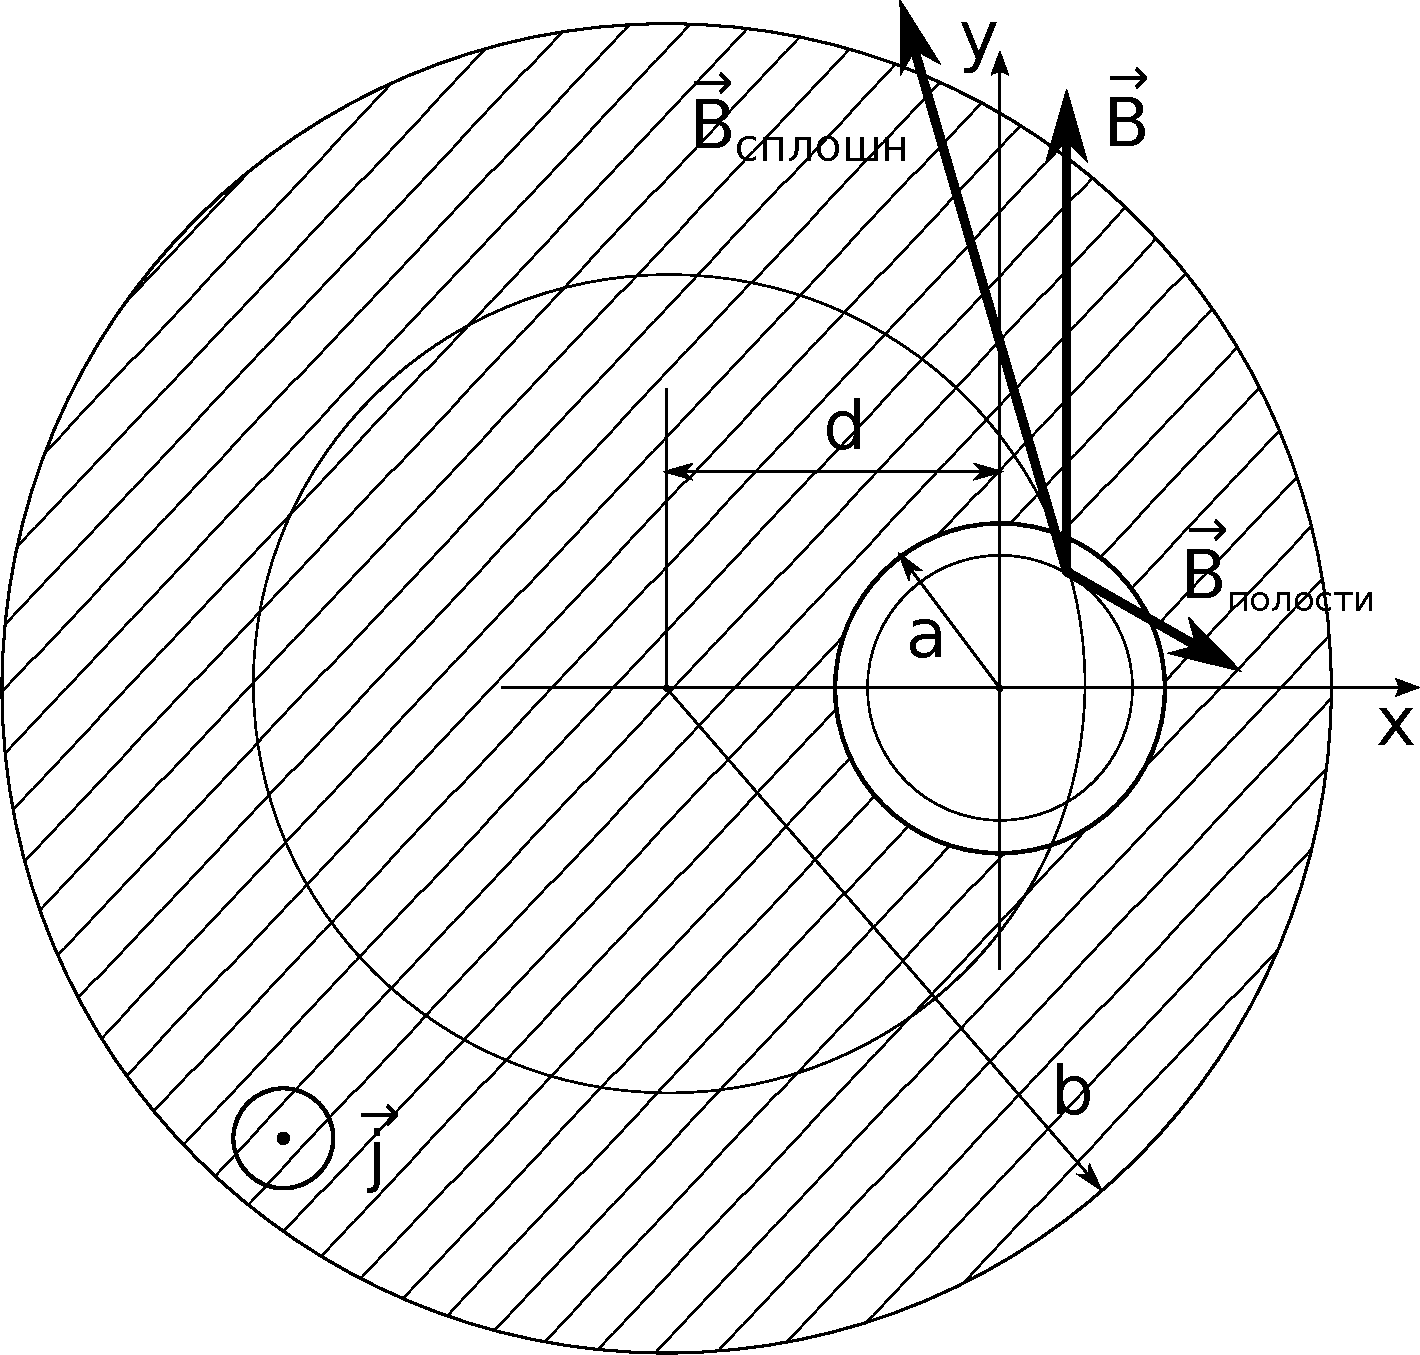
\includegraphics[width=.4\textwidth]{1-2}
\end{figure}
\emph{Решение:}
Ток, текущий по проводнику с полостью можно рассматривать как суперпозицию
двух токов той же плотности: тока, сонаправленного с ним и текущего по
проводнику с заполненной полостью и противоположно направленного тока
полости. Плотность каждого из токов равна
\[
    j = \frac{I}{\pi(b^2 - a^2)}.
\]
Тогда во введёной на рисунке системе координат поля внутри полости имеют вид
\[
    \vec{B}_\textit{полости} = \frac{\mu_0j}{2}\{y, -x, 0\} \text{ и }
    \vec{B}_\textit{сплошн} = \frac{\mu_0j}{2}\{-y, x+d, 0\}.
\]
Их суперпозиция даёт фактическое поле внутри полости \( \vec{B} \):
\[
    \vec{B} = \vec{B}_\textit{полости} + \vec{B}_\textit{сплошн} =
    \frac{\mu_0j}{2}\{0, d, 0\} = \frac{\mu_0 I d}{2\pi(b^2 - a^2)}\{0, 1, 0\}.
\]
Таким образом, магнитное поле внутри полости является однородным.
\vfill
\emph{Ответ:}
\[
    \vec{B} = \left\{0, \frac{\mu_0 I d}{2\pi(b^2 - a^2)}, 0\right\}.
\]

\newpage
%-------------------------------------------------------------------------------
\emph{549.} <<Поезд>> \( A'B' \), длина которого \( l_0 = 8,64 \cdot 10^8 \)~км
в системе, где он покоится, идет со скоростью \( \v = 240 000 \)~км/сек мимо
<<платформы>>, имеющей такую же длину в своей системе покоя. В голове \( B' \) и
хвосте \( A' \) <<поезда>> имеются одинаковые часы, синхронизованные между
собой. Такие же часы установлены в начале \( (A) \) и в конце \( (B) \)
<<платформы>>. В тот момент, когда голова <<поезда>> поравнялась с началом
<<платформы>>, совпадающие часы показывали 12~час~00~мин. Ответить на
следующие вопросы:
\vspace*{-.9em}
\begin{enumerate} \itemsep-.5em
    \item можно ли утверждать, что в этот момент в какой-либо системе отсчета все
    часы также показывают 12~час~00~мин;
    \item сколько показывают каждые из часов в момент, когда хвост <<поезда>>
    поравнялся с началом <<платформы>>;
    \item сколько показывают часы в момент, когда голова «поезда» поравнялась
    с концом <<платформы>>?
\end{enumerate}

\vspace*{2em}
\emph{Решение:}
\begin{enumerate}
    \item Чтобы ответить на этот вопрос рассмотрим понятие одновременности. Если
    в момент времени \( t_A \) (по часам в точке \( A \)) луч света выходит из
    точки \( A \), идет в точку \( B \), отражается в момент \( t_B \) (по часам
    в точке \( B \)), идет обратно в точку \( A \) и возвращается в момент
    времени \( t_A' \) (по часам в точке \( A \)). Часы в \( A \) и \( B \)
    будут идти, согласно определению, синхронно, если выполняется условие:
    \[
        t_B - t_A = t_A' - t_B.
    \]
    Это время в покоящейся системе отсчета -- на платформе.
    
    Рассмотрим движущийся поезд. Если в момент времени \( t_{A'} \) из точки
    \( A' \) выходит луч света, отражается в точке \( B' \) в момент времени
    \( t_{B'} \) и возвращается в точку \( A' \) в момент времени \( t_{A'}' \).
    Принимая во внимание принцип постоянства скорости света, находим:
    \[
        t_{B'} - t_{A'} = \frac{l_0}{\v - v}; \quad t_{A'}' - t_{B'} = \frac{l_0}{\v + v},
    \]
    где \( l_0 \) -- собственная длина поезда.
    
    Таким образом, видно, что время не будет одинаковым на всех часах:
    для наблюдателя, находящегося на платформе, время будет идти синхронно лишь
    на часах на платформе; для наблюдателя, находящегося в поезде, время будет
    идти синхронно лишь для часов в поезде.
    
    \item Рассмотрим случай, когда хвост поезда поравнялся с началом платформы.
    
    Находясь в поезде, время изменится на величину \( \d t \), равную времени,
    за которое поезд пройдет расстояние \( l_0 \):
    \[
        \d t = l_0/\v = 1 \text{ час}.
    \]
    Таким образом, время в точке \( t_{A'} = 12^{00} + 1^{00} = 13^{00} \).
    
    Время, которое показывают часы в начале платформы, вычислим, учитывая
    лоренцево преобразование времени:
    \[
        \d t' = \d t \sqrt{1 - (\v/c)^2} = \frac{l_0}{\v} \cdot \sqrt{1 -
        \left(\frac{\v}{c}\right)^2}.
    \]
    Откуда \( t_A = 12^{36} \).
    
    Теперь рассмотрим показание часов в начале поезда \( B' \) и в конце
    платформы \( B \). Находясь в разных системах отсчета, часы не будут идти
    синхронно.
    
    \begin{figure}[h!]
        \center
        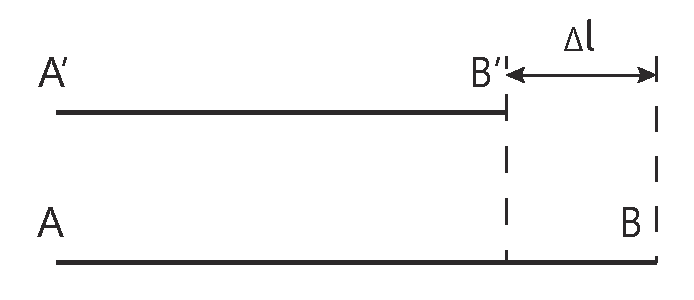
\includegraphics[width = .4\textwidth]{1-3_1-1}\hspace*{2em}
        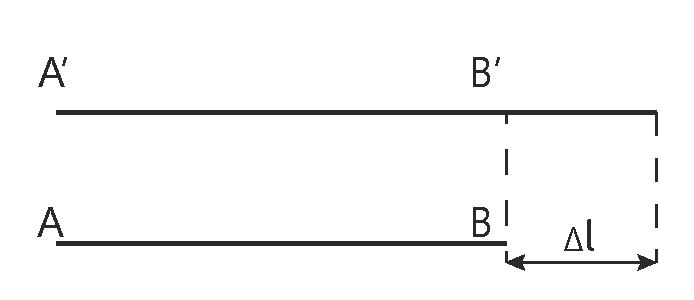
\includegraphics[width = .4\textwidth]{1-3_1-2} \\
        \parbox{.4\textwidth}{\centering Наблюдатель на платформе}\hspace*{2em}
        \parbox{.4\textwidth}{\centering Наблюдатель в поезде}
    \end{figure}
    
    Рассмотрим случай, когда наблюдатель находится на платформе. В таком случае
    часы, находящиеся в конце платформы будут показывать то же время, что часы в
    начале платформы:
    \[
        t_B = t_A = 12^{36}.
    \]
    В начале поезда время на часах будет отличным от того, что показывают часы в
    конце поезда. Для наблюдателя длина поезда будет короче, чем длина
    платформы. В таком случае, учитывая разницу в длине:
    \[
        \d l = l_0 - l_0 \cdot \sqrt{1 - \left(\frac{\v}{c}\right)^2},
    \]
    рассчитаем время в точке \( B' \):
    \[
        \d t = \frac{\d l}{\v} = 14,\!4 \text{ мин}; \quad t_{B'} = t_B - \d t =
        12\text{ час } 21,\!6 \text{ мин}.
    \]
    
    Теперь рассмотрим случай, когда наблюдатель находится в поезде. В этом
    случае часы в поезде синхронизированы и показывают одно время:
    \[
        t_{B'} = t_{A'} = 13^{00}.
    \]
    
    Теперь длина платформы будет казаться меньше:
    \[
        \d l = l_0 - l_0 \cdot \sqrt{1 - \left(\frac{\v}{c}\right)^2}; \quad
        \d t = \frac{\d l}{\v} = 14,\!4 \text{ мин}.
    \]
    Тогда время в точке \( B \):
    \[
        t_B = t_{B'} + \d t = 13 \text{ час } 14,\!4 \text{ мин}.
    \]
    
    \item Рассмотрим случай, когда начало поезда поравнялось с концом платформы.
    
    \begin{figure}[h!]
        \center
        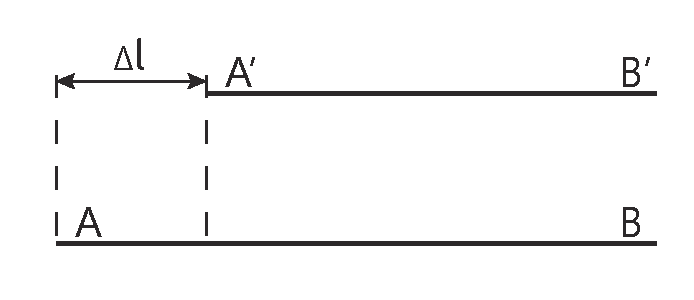
\includegraphics[width = .4\textwidth]{1-3_2-1}\hspace*{2em}
        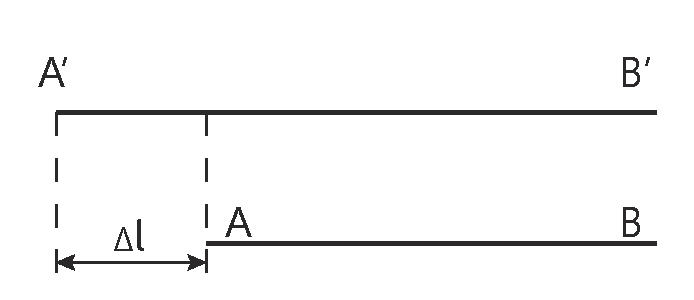
\includegraphics[width = .4\textwidth]{1-3_2-2} \\
        \parbox{.4\textwidth}{\centering Наблюдатель на платформе}\hspace*{2em}
        \parbox{.4\textwidth}{\centering Наблюдатель в поезде}
    \end{figure}
    
    Для наблюдателя, находящегося на платформе (значение \( \d t = 14,4 \)~мин
    было найдено ранее):
    \begin{align*}
        & t_A = t_B = 12^{36} + \d t = 13^{00}; \\
        & t_{A'} = 13^{00} + \d t = 13\text{ ч } 14,\!4 \text{ м}; \\
        & t_{B'} = 12\text{ ч } 21,\!6 \text{ м} + \d t = 12^{36}.
    \end{align*}
    
    Для наблюдателя, находящегося в поезде:
    \begin{align*}
        & t_{A'} = t_{B'} = 12^{00} + \frac{l_0}{\v} \cdot \sqrt{1 -
        \left(\frac{\v}{c}\right)^2} = 12^{36}; \\
        & t_B = 12^{00} + \frac{l_0}{\v} = 13^{00}; \\
        & t_A = t_{A'} - \d t = 12\text{ ч } 21,\!6 \text{ м}.
    \end{align*}
\end{enumerate}
\vspace*{2em}
\emph{Ответ:} а) Нельзя; \ \ б) \( t_{A'} = 13^{00} \), \( t_A = 12^{36} \),

для наблюдателя на платформе: \( t_{B'} = 12^{21,6} \), \( t_B = 12^{36} \),

для наблюдателя в поезде: \( t_{B'} = 13^{00} \), \( t_B = 13^{14,4} \);

в) для наблюдателя на платформе: \( t_{A'} = 13^{14,4} \), \( t_{B'} = 12^{36} \),
\( t_A = t_B = 12^{36} \),

для наблюдателя в поезде: \( t_{A'} = t_{B'} = 12^{36} \), \( t_A = 12^{21,6} \),
\( t_B = 13^{00} \).
\end{document}
